\documentclass{article} % For LaTeX2e
\usepackage{iclr2015,times}
\usepackage{hyperref} % For clickable links (internal/external)
\usepackage{url} % For formatting web links
\usepackage{natbib} % Might be iclr specific
\usepackage{amsmath} % Nice math
\usepackage{amssymb} % More nice math
\usepackage{graphicx} % Import images
\usepackage{subfig} % If you want subfigures
\usepackage{wrapfig} % Wrap text arounf figures

\title{Title of the paper}

\newcommand*\samethanks[1][\value{footnote}]{\footnotemark[#1]}

\author{
Tom Le Paine\thanks{ - Authors contributed equally to this work.}, Pooya Khorrami\samethanks, Wei Han, Thomas S. Huang \\
Beckman Institute for Advanced Science and Technology,\\
University of Illinois at Urbana-Champaign\\
Urbana, IL 61801\\
\texttt{{paine1,pkhorra2,weihan3,t-huang1}@illinois.edu} \\
}


\newcommand{\fix}{\marginpar{FIX}}
\newcommand{\new}{\marginpar{NEW}}

\begin{document}

\maketitle

% Abstract
\begin{abstract}
Abstract.
\end{abstract}

% Paper sections
\section{Introduction}
\label{sec:intro}
For starters (\citet{krizhevsky2012imagenet}).

% Give outline of the paper
In Section \ref{sec:method}, we will present our method, we present experiments in Section \ref{sec:experiments}, and in Section \ref{sec:conclusions} we conclude the paper.

\section{Related Work}
\label{sec:related_work}
Related work.










\section{Our Approach}
\label{sec:method}
\subsection{Subsection}
% Highlight differences
Inline equations $E_{l}(\cdot)$.

\begin{equation}
E_{l}(x) = P_{s_l}f(F_{l}x)
\label{eq:encoder}
\end{equation}

\begin{gather}
C_1(x) = \| x - D_{1}(E_{1}(x)) \|_{2}^{2} \\
C_2(x) = \| x - D_{1}(D_{2}(E_{2}(E_{1}(x)))) \|_{2}^{2}
\label{eq:layer_cost}
\end{gather}

\section{Experiments and Analysis}
\label{sec:experiments}
\subsection{Subsection}

Figure reference: \ref{fig:name}.

\begin{wrapfigure}{R}{0.5\textwidth}
\centering
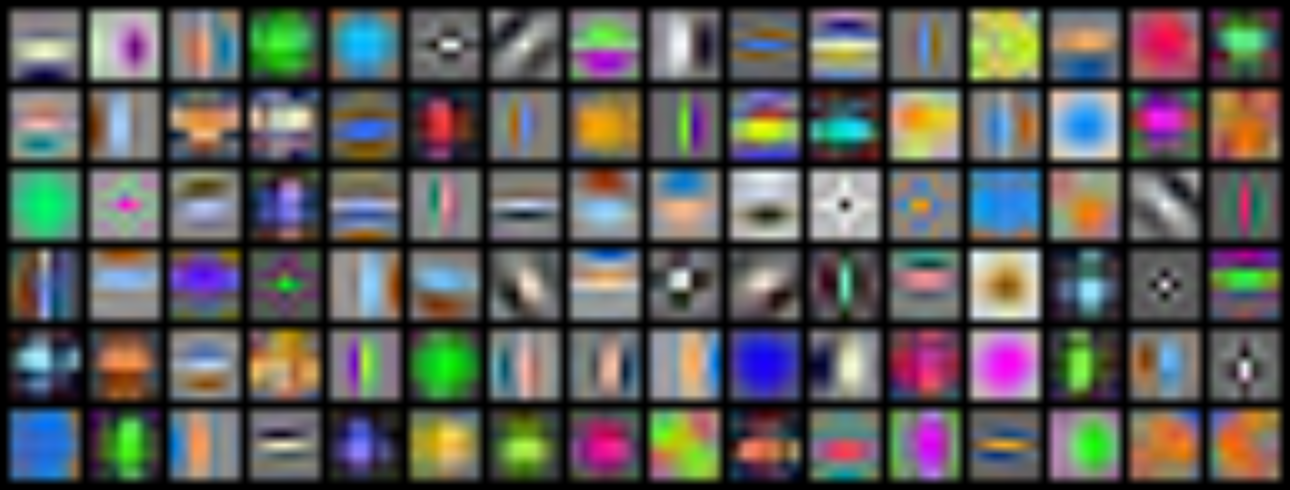
\includegraphics[width=0.48\textwidth]{./figures/cifar10_layer1_filters_7x7_11m-09d-21h-38m-00s.png}
\caption{Caption.}
\label{fig:name}
\vspace{-0.5cm}
\end{wrapfigure}

Table reference: \ref{tab:name}

\begin{table}[b]
\begin{center}
    \caption{Table.}
    \label{tab:name}
    \begin{tabular}{ |l | c | c | c | c |}
    \hline
    \multicolumn{1}{|p{5cm}|}{\raggedright Unsupervised to supervised ratio \\ (Samples per Class)}
& \multicolumn{1}{|p{1cm}|}{\centering 50:1 \\ (100)}
& \multicolumn{1}{|p{1cm}|}{\centering 10:1 \\ (500)}
& \multicolumn{1}{|p{1cm}|}{\centering 5:1  \\ (1000)}
& \multicolumn{1}{|p{1cm}|}{\centering 1:1  \\ (5000)} \\ \hline
     Tanh CNN & 44.48 \% & --- & 64.77 \% & 77.50 \% \\ %\hline
     Tanh CAE & 47.70 \% & --- & 65.65 \% & 78.20 \% \\ \hline
     Zero-bias CNN  & 47.01 \% & 64.76 \%& 73.30 \% & 82.73 \% \\
     \bf Zero-bias CAE  & \bf 55.45 \% & \bf 68.42 \% & \bf 74.06 \% & \bf 83.64 \% \\ \hline
    \end{tabular}
\end{center}
\end{table}

\section{Conclusions}
\label{sec:conclusions}
Conclusion.

\subsubsection*{Acknowledgments}
\label{sec:conclusions}
Acknowledgement.

\bibliography{main}
\bibliographystyle{plainnat}


\end{document}